\section{The simulation engine}
\label{sec:simulation}

A relational-event model is only as testable as the data-generating
process one can pair with it. \pkg{amore} therefore ships a first-class
forward simulator, \texttt{simulate\_relational\_events()}, alongside the
estimation machinery. The simulator is not an afterthought: it is the
ground-truth oracle behind every recovery experiment in
Section~\ref{sec:validation}, and its output is shaped so that it feeds
\texttt{rem()} without an intervening reshaping step. This section
describes the two driving algorithms (exact Gillespie and approximate
$\tau$-leap), the five generative mechanisms they compose, the
ready-to-fit case--control output, the measured scaling behaviour, and the
companion hyperedge (RHEM) simulators.

\subsection{One front door, five composable mechanisms}
\label{sec:sim-mechanisms}

\texttt{simulate\_relational\_events()} exposes a single entry point that
layers five mechanisms on top of an event-by-event inner loop. Each
mechanism is opt-in through its own arguments and the mechanisms compose
freely:

\begin{enumerate}
\item \textbf{A homogeneous baseline.} A positive \texttt{baseline\_rate}
  multiplies the hazard of every admissible dyad, giving the minimal
  memoryless process \citep{butts2008}.
\item \textbf{Per-dyad contribution logits.} A static $S \times R$ matrix
  \texttt{contribution\_logits} adds a dyad-specific term to the log-rate
  --- for example inter-state distances, role similarities, or a planted
  non-linear surface $f(x_{sr})$ (used to stress smooth recovery in
  experiment E2 of Section~\ref{sec:validation}).
\item \textbf{Exogenous actor covariates.} Per-actor numeric tables
  (\texttt{sender\_covariates}, \texttt{receiver\_covariates}) with their
  effect vectors enter the linear predictor additively. The companion
  generator \texttt{simulate\_actor\_covariates()} produces either static
  per-actor attributes or time-stamped AR(1) processes for repeated
  exogenous draws.
\item \textbf{Endogenous statistics.} Any subset of the endogenous
  catalogue (Section~\ref{sec:statistics}) can be activated through
  \texttt{endogenous\_stats} / \texttt{endogenous\_effects}; the simulator
  maintains the corresponding state matrices and updates them after every
  fired event, so the intensity of the next event depends on the realized
  history. This is the formulation of \citet{juozaitiene2024}.
\item \textbf{Time-varying global covariates.} A piecewise-constant grid
  (\texttt{global\_covariates} with a \texttt{time\_start} column, and
  \texttt{global\_effects}) rescales the total event rate by
  $\exp\!\big(\sum_k \beta_k\, x_k(t)\big)$. Because the multiplier is the
  same for every dyad, it cancels from the per-dyad selection
  probabilities and acts only on the waiting-time distribution --- the
  identifiability structure exploited by the time-shift sampling of
  \citet{lembo2025}.
\end{enumerate}

The same five-mechanism state machine drives both algorithms, so a model
specified once can be simulated under either scheme without change.

\subsection{Gillespie and \texorpdfstring{$\tau$}{tau}-leap}
\label{sec:sim-algorithms}

The default algorithm is the exact event-driven Gillespie scheme
\citep{gillespie1977}: at each step the simulator computes every dyad's
current intensity, draws the inter-event waiting time from an exponential
with rate equal to the sum of all dyadic intensities, and selects the
firing dyad with probability proportional to its intensity (a softmax over
the risk set). Because the full risk set is recomputed after every event,
Gillespie is exact but per-event in cost.

When global covariates are active the simulator switches to a
\emph{boundary-aware} Gillespie variant: whenever a sampled waiting time
would carry the clock across an interval boundary of the
piecewise-constant grid, the clock is advanced to the boundary without
recording an event and the next waiting time is redrawn under the new
global multiplier. This keeps the inhomogeneous process exact rather than
approximating it on the grid.

The alternative is \texttt{method = "tau\_leap"}, a time-driven
approximation. It advances the clock by a fixed step $\tau$ and, for every
dyad, draws a $\mathrm{Poisson}(\lambda_{sr}(t)\,\tau)$ number of events
using the rates at the \emph{start} of the step; events that fire within a
step are placed at uniform times in $[t, t+\tau)$, reported in time order,
and share the start-of-step state, which is then updated once at the end
of the step. The $\tau$-leap scheme trades exactness for predictable,
vectorised work per step and is stated honestly as an approximation: it
converges in distribution to the exact Gillespie result only as
$\tau \to 0$. Practical use requires $\lambda\tau \ll 1$ on every active
dyad and $\tau$ smaller than the shortest global-covariate interval
(within-step boundary crossings are not resolved).

\subsection{Risk-set rule and ready-to-fit output}
\label{sec:sim-output}

Two further controls make the simulator a direct estimation companion
rather than a bare event generator.

\textbf{Risk-set rule.} \texttt{risk = "standard"} (the default) keeps
every dyad eligible at every step. \texttt{risk = "remove"} drops a dyad
from the risk set as soon as it fires, mimicking one-shot processes such
as species invasions or first-citation events, where a dyad cannot repeat.

\textbf{Case--control output.} Setting \texttt{n\_controls = k} emits a
stratified case--control table directly: each realized event becomes one
\emph{case} row paired with $k$ \emph{control} rows sampled from the
non-event risk set at that moment, all sharing a \texttt{stratum}
identifier, with an \texttt{event} indicator (1 for the case, 0 for
controls). When endogenous statistics or global covariates are active, the
value each row's dyad carried at its event time is appended as a column,
so a downstream conditional-logistic or GAM fit recovers the planted
effects. This is the sampled-risk-set reduction of \citet{lerner2020}
produced at generation time.

For the common case-1-control design, \texttt{wide = TRUE} (which requires
\texttt{n\_controls = 1}) reshapes the long table to one row per event,
carrying the event-dyad actors (\texttt{sender\_ev},
\texttt{receiver\_ev}), the matched control-dyad actors
(\texttt{sender\_nv}, \texttt{receiver\_nv}), and for each covariate the
event value (\texttt{<cov>\_ev}), the control value (\texttt{<cov>\_nv}),
and their difference (\texttt{d\_<cov>}). The difference columns are
exactly the design matrix of the degenerate case-1-control logistic
regression fitted by the \texttt{gam} backend
(Section~\ref{sec:framework}), so the simulator's output is ready to fit
with no further preparation:

\begin{verbatim}
wide_events <- simulate_relational_events(
  n_events           = 5,
  senders            = LETTERS[1:3],
  receivers          = LETTERS[1:3],
  n_controls         = 1,
  endogenous_stats   = "reciprocity_count",
  endogenous_effects = c(reciprocity_count = 0.6),
  wide               = TRUE)
\end{verbatim}

\subsection{Scaling: when to leap}
\label{sec:sim-scaling}

Experiment E4 of Section~\ref{sec:validation} times both algorithms over a
$4 \times 5 \times 2$ grid
(\texttt{n\_actors} $\in \{15, 30, 60, 100\}$,
\texttt{n\_events} $\in \{500, 1000, 2500, 5000, 10000\}$, both methods,
$\tau = 0.05$), on a single reciprocity term with no case--control
sampling so the wall-clock isolates the simulator. Absolute seconds are
machine-specific (Apple Silicon M1 Max); the scaling shape and ratios are
what transfer.

On the stable cells, $\tau$-leap is \textbf{22--42$\times$ faster than
Gillespie at \texttt{n\_actors} $= 60$} and \textbf{37$\times$ to
$\approx 100\times$ faster at \texttt{n\_actors} $= 100$}, the gap widening
with \texttt{n\_events} (Gillespie recomputes the full risk set per event;
$\tau$-leap takes vectorised Poisson leaps). At 10,000 events the
100-actor cell runs in $\approx 3.4$\,s under Gillespie and
$\approx 0.033$\,s under $\tau$-leap. Figure~\ref{fig:exp4-scaling}
plots the full grid.

\begin{figure}[t]
\centering
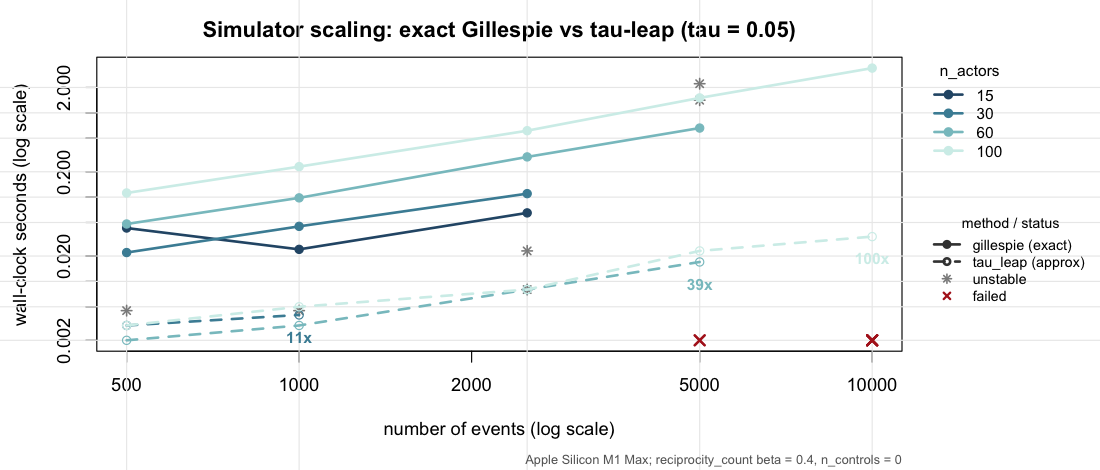
\includegraphics[width=0.9\textwidth]{figs/exp4-scaling.png}
\caption{Simulator wall-clock scaling (experiment E4). $\tau$-leap
(dashed) bundles events into fixed time slices and scales markedly better
than the exact per-event Gillespie scheme (solid) as the actor universe
grows, reaching $\approx 100\times$ at 100 actors and 10{,}000 events.
Absolute times are machine-specific; the ratios transfer. Cells that fall
in the small-network failure regime are omitted.}
\label{fig:exp4-scaling}
\end{figure}

We report the failure regime as plainly as the speed-ups, because both
back-ends break down at \emph{small} \texttt{n\_actors} under a strongly
self-exciting reciprocity process, for opposite reasons. Gillespie's
per-dyad softmax underflows (``too few positive probabilities'') at
\texttt{n\_actors} $\in \{15, 30\}$ for \texttt{n\_events} $\ge 5000$ (and
at 60 actors for 10,000 events): the self-excitation concentrates almost
all probability mass on a few reciprocating dyads, and the remaining
intensities round to zero. The $\tau$-leap intensities instead explode
into a memory blow-up (seed-dependent at small sizes; all replicates fail
at 10,000 events for \texttt{n\_actors} $\le 60$). At 10,000 events only
the 100-actor cell is clean for both methods. The practical guidance is
to use Gillespie for small or dense networks where exactness is cheap, to
use $\tau$-leap for large actor universes where wall-clock matters, and in
the high-rate small-network corner to reduce the self-exciting effect
size, raise the actor count, or validate $\tau$ against a short Gillespie
run before trusting it. None of these limits is silent: each failure
surfaces as an error rather than a wrong number.

\subsection{Hyperedge and RHEM simulators}
\label{sec:sim-hyperedge}

For relational \emph{hyper}-events --- where senders and receivers are
\emph{sets} of actors rather than single actors --- \pkg{amore} ships three
companion simulators that follow the formulation of
\citet{boschi2025rhem}. \texttt{simulate\_hyperedge\_events()} generates
\emph{undirected} multi-actor meetings (subsets of the actor set of size up
to \texttt{max\_size}), matching Section~4 of that paper.
\texttt{simulate\_directed\_hyperedge\_events()} generates \emph{directed}
two-mode hyperevents from a sender set $I_m$ to a receiver set $J_m$ (both
non-empty), the data model of Section~5 for citation networks. Both fire a
candidate hyperedge $(I, J)$ with rate
$\lambda(t, I, J) = \lambda_0 \exp\!\big(\sum_k \beta_k\, x_k(t, I, J)\big)$
and draw waiting times from an exponential with the total intensity ---
the same Gillespie logic as the dyadic engine, lifted to set-valued
events. The supported hyperedge statistics are the cardinality terms
(\texttt{size}, \texttt{size\_I}, \texttt{size\_J}), past-event
\texttt{activity}, and directed/undirected \emph{subset repetition}
\texttt{subrep\_<$\rho$>} (paper eq.~4), the mechanism by which a recurring
subset of participants raises the rate of future hyperedges that contain
it. Figure~\ref{fig:hyper-running-subrep} illustrates a subset-repetition
driven directed hyperevent stream.

Because each step enumerates every candidate hyperedge, the candidate
space is exponential in the universe size; these simulators are therefore
explicitly bounded to small actor / item universes (practically
$|V| \le 20$ with small maximum cardinality), and the documentation states
this limit. The third simulator,
\texttt{simulate\_directed\_hyperevents\_tvnl()}, is a teaching-oriented
generator with a \emph{time-varying} sender effect $\alpha(t)$ and a
\emph{non-linear} receiver effect $f(x)$, intended for demonstrating
GAM-based recovery of smooth (TV/NL) effects. It attaches the ground-truth
$\alpha(t)$ and $f(x)$ as \texttt{attr(., "truth")} on its output so a
fitted smooth can be compared directly against the function that generated
it.

\begin{figure}[t]
\centering
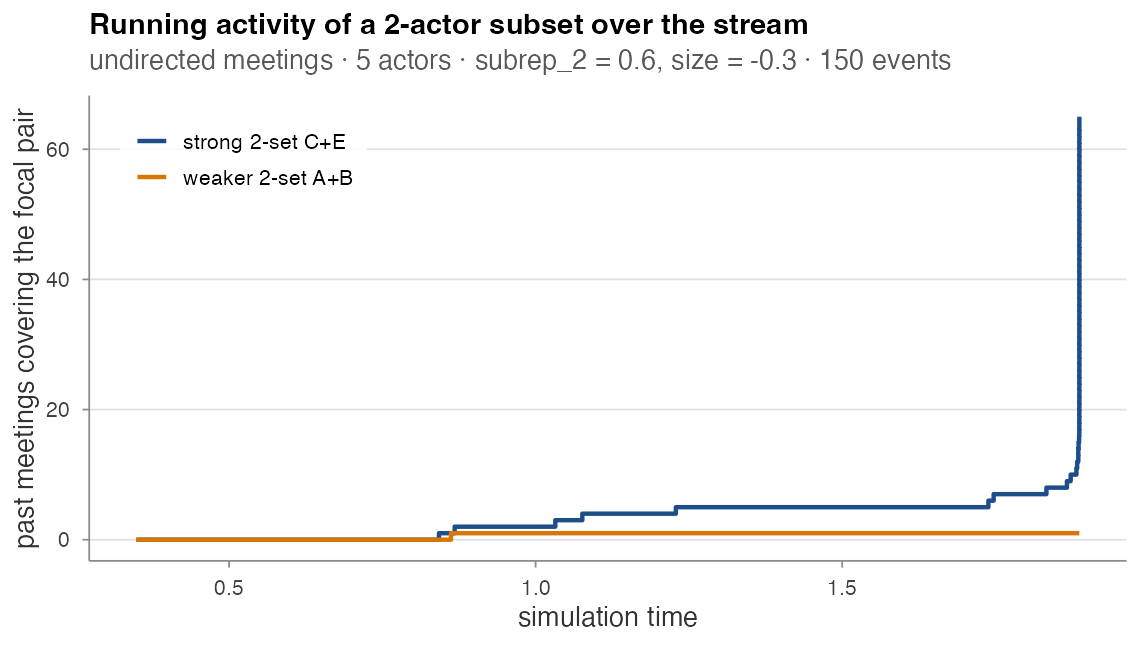
\includegraphics[width=0.7\textwidth]{figs/hyper-running-subrep.png}
\caption{A directed hyperevent stream simulated under a positive subset
repetition (\texttt{subrep}) effect: recurring participant subsets raise
the intensity of future hyperedges that contain them
\citep{boschi2025rhem}. The hyperedge simulators reuse the dyadic engine's
Gillespie logic over set-valued candidates.}
\label{fig:hyper-running-subrep}
\end{figure}

The hyperedge simulators produce hyperedge logs and case--control
hyperedge features; they exercise the full RHEM feature path. We note for
honesty that no bundled vignette yet carries a hyperedge stream all the way
through an end-to-end \texttt{rem()} fit --- the RHEM features are
\texttt{rem}-ready but the closed-loop demonstration on hyperevent data is
left to future work.
